\documentclass{article}%
\usepackage[T1]{fontenc}%
\usepackage[utf8]{inputenc}%
\usepackage{lmodern}%
\usepackage{textcomp}%
\usepackage{lastpage}%
%
\usepackage{amsmath}%
\usepackage{amssymb}%
\usepackage{amsfonts}%
\usepackage{graphicx}%
\usepackage{hyperref}%
\usepackage{tikz}%
\usepackage{pgfplots}%
\usetikzlibrary{math}%
\title{IME 2026 - Química\thanks{This exam was solved and automatically generated with gpt-resolve: \url{https://github.com/lgabs/gpt-resolve}}}%
\author{claude{-}opus{-}5{-}5 (solver) + claude{-}opus{-}5{-}5 (judge)}%
\date{November 10, 2026}%
%
\begin{document}%
\normalsize%
\maketitle%
\section*{Questão 1}

\section*{Solução}

\textbf{Hipóteses.} A eletrólise ígnea tem rendimento de corrente de 100\% (toda a carga que passa é usada na redução do cátion metálico), e a corrente é constante durante todo o processo.

\textbf{1) Carga que circulou.} Com a corrente constante, $Q = i\,\Delta t$, e o tempo deve estar em segundos:
\[
\Delta t = 6{,}7\ \text{h}\times 3600\ \tfrac{\text{s}}{\text{h}} = 24120\ \text{s},
\qquad
Q = 0{,}4\ \text{A}\times 24120\ \text{s} = 9648\ \text{C}.
\]

\textbf{2) Quantidade de elétrons (1ª lei de Faraday).} Um mol de elétrons transporta $F = 96480\ \text{C}$:
\[
n_{e^-} = \frac{Q}{F} = \frac{9648\ \text{C}}{96480\ \text{C}\cdot\text{mol}^{-1}} = 0{,}100\ \text{mol}.
\]

\textbf{3) Estequiometria no cátodo.} No sal $\text{MC}\ell_2$, eletricamente neutro, cada $\text{C}\ell^-$ tem carga $-1$, logo o cátion é $\text{M}^{2+}$. No sal fundido:
\[
\text{cátodo: } \text{M}^{2+} + 2e^- \longrightarrow \text{M}(s), \qquad
\text{ânodo: } 2\,\text{C}\ell^- \longrightarrow \text{C}\ell_2(g) + 2e^-.
\]
Assim, cada mol de M depositado consome 2 mol de elétrons:
\[
n_{\text{M}} = \frac{n_{e^-}}{2} = 0{,}050\ \text{mol}.
\]

\textbf{4) Massa molar de M.}
\[
\mathcal{M}_{\text{M}} = \frac{m}{n_{\text{M}}} = \frac{4{,}38\ \text{g}}{0{,}050\ \text{mol}} = 87{,}6\ \text{g}\cdot\text{mol}^{-1}.
\]

\textbf{5) Identificação.} Na tabela fornecida, o elemento de massa atômica $87{,}62$ é o \textbf{estrôncio} (Sr, $Z = 38$). A massa de 87{,}6 não coincide com a de nenhum vizinho próximo: Rb (85{,}47) e Y (88{,}91).

\textbf{Verificação de consistência.} O Sr é um metal alcalino-terroso (grupo 2). Ele forma apenas o cátion $\text{Sr}^{2+}$ e, portanto, o cloreto $\text{SrC}\ell_2$, o que concorda com a fórmula $\text{MC}\ell_2$ do enunciado. Por ser muito reativo, o Sr metálico é obtido justamente por eletrólise do sal fundido, e não em solução aquosa, onde a água seria reduzida em seu lugar. Quanto às unidades, $\text{A}\cdot\text{s} = \text{C}$ e $\text{C}/(\text{C}\cdot\text{mol}^{-1}) = \text{mol}$; a ordem de grandeza ($0{,}05$ mol, cerca de 4 g) é coerente.

\medskip
\noindent ANSWER: O metal M é o estrôncio (Sr, $Z = 38$), com $\mathcal{M} = 4{,}38/0{,}050 = 87{,}6\ \text{g}\cdot\text{mol}^{-1}$ (sal $\text{SrC}\ell_2$).%
\newpage%
\section*{Questão 2}

\section*{Solução}

\textbf{1) O que cada informação revela.}
\begin{itemize}
\item A ($\mathrm{C_5H_{11}C\ell}$) é um haleto de alquila saturado e acíclico ($\mathrm{C_nH_{2n+1}X}$). A desidro-halogenação (eliminação de HC$\ell$, p.\,ex.\ com KOH em etanol, a quente) gera um alceno B de fórmula $\mathrm{C_5H_{10}}$.
\item A ozonólise ($\mathrm{O_3}$, seguida de $\mathrm{H_2O/Zn}$) quebra a ligação $\mathrm{C=C}$ e transforma cada carbono da dupla em carbonila. Só se forma formaldeído ($\mathrm{HCHO}$) a partir de um grupo $\mathrm{=CH_2}$; logo, B tem a \textbf{dupla terminal} ($\mathrm{CH_2=C\ldots}$).
\item A hidratação ácida de alcenos segue a regra de Markovnikov (o H vai para o carbono mais hidrogenado, o OH vai para o carbono que forma o carbocátion mais estável). O produto C é um álcool.
\item O $\mathrm{KMnO_4}$ em meio ácido oxida álcoois primários (a aldeído/ácido carboxílico) e secundários (a cetona), porque o carbono que tem o OH possui H. O álcool \textbf{terciário} não tem H nesse carbono e por isso não reage. Logo, C é um álcool terciário.
\end{itemize}

\textbf{2) Escolha de B.} Os alcenos $\mathrm{C_5H_{10}}$ de dupla terminal e os álcoois que dão por hidratação (Markovnikov):
\[
\begin{array}{lll}
\mathrm{CH_2=CHCH_2CH_2CH_3} & \to\ \mathrm{CH_3CH(OH)CH_2CH_2CH_3} & \text{(secundário: oxida)}\\[2pt]
\mathrm{CH_2=CHCH(CH_3)_2} & \to\ \mathrm{CH_3CH(OH)CH(CH_3)_2} & \text{(secundário: oxida)}\\[2pt]
\mathrm{CH_2=C(CH_3)CH_2CH_3} & \to\ \mathrm{(CH_3)_2C(OH)CH_2CH_3} & \text{(terciário: não oxida)}
\end{array}
\]
Só o 2-metilbut-1-eno satisfaz as duas condições. Nesta análise usamos a adição de Markovnikov direta, sem rearranjo de carbocátion, como é usual. Portanto
\[
\text{B: } \mathrm{H_2C=C(CH_3)-CH_2-CH_3}\quad\text{(2-metilbut-1-eno)}.
\]
Confirmação (formam-se formaldeído e butanona):
\[
\mathrm{H_2C=C(CH_3)CH_2CH_3 \xrightarrow{\ O_3;\ H_2O/Zn\ } HCHO + CH_3COCH_2CH_3}
\]

\textbf{3) Composto C.}
\[
\mathrm{H_2C=C(CH_3)-CH_2-CH_3 + H_2O \xrightarrow{\ H^+\ } CH_3-C(OH)(CH_3)-CH_2-CH_3}
\]
C é o 2-metilbutan-2-ol ($\mathrm{C_5H_{12}O}$), um álcool terciário: a hidroxila fica num carbono ligado a três outros carbonos. Esse carbono não tem H, então C não é oxidado pelo $\mathrm{KMnO_4/H^+}$.

\textbf{4) Composto A.} O cloreto precisa ter o esqueleto do 2-metilbutano, com o C$\ell$ num dos carbonos da futura dupla (C1 ou C2):
\begin{itemize}
\item \emph{2-cloro-2-metilbutano}: tem dois carbonos $\beta$ com H (C1 e C3). Pela regra de Saytzeff, o produto principal é o alceno mais substituído, o 2-metilbut-2-eno $\mathrm{(CH_3)_2C=CH-CH_3}$. Sua ozonólise dá acetona e acetaldeído, sem formaldeído. Por isso esse cloreto não forma B de modo inequívoco.
\item \emph{1-cloro-2-metilbutano}: o único carbono $\beta$ é o C2, que tem um só H. Assim, a eliminação só pode formar a dupla C1=C2, e B é o \textbf{único} produto (o HC$\ell$ eliminado é neutralizado pela base):
\[
\mathrm{C\ell CH_2CH(CH_3)CH_2CH_3 \xrightarrow{\ KOH/etanol,\ \Delta\ } H_2C=C(CH_3)CH_2CH_3 + HC\ell}
\]
\end{itemize}
Logo, A é o 1-cloro-2-metilbutano. A fórmula confere: $\mathrm{C_5H_{11}C\ell}$, com $2+1+3+2+3=11$ hidrogênios. Seu C2 é quiral (ligado a H, $\mathrm{CH_3}$, $\mathrm{C_2H_5}$ e $\mathrm{CH_2C\ell}$), mas a pergunta pede só a fórmula estrutural.

\textbf{Respostas.}

a) C é um \textbf{álcool} (álcool terciário).

b)
\[
\begin{aligned}
\text{A}&:\ \mathrm{C\ell-CH_2-CH(CH_3)-CH_2-CH_3}\ \text{(1-cloro-2-metilbutano)}\\
\text{B}&:\ \mathrm{H_2C=C(CH_3)-CH_2-CH_3}\ \text{(2-metilbut-1-eno)}\\
\text{C}&:\ \mathrm{CH_3-C(OH)(CH_3)-CH_2-CH_3}\ \text{(2-metilbutan-2-ol)}
\end{aligned}
\]

ANSWER: a) álcool (terciário); b) A = 1-cloro-2-metilbutano, $\mathrm{C\ell CH_2CH(CH_3)CH_2CH_3}$; B = 2-metilbut-1-eno, $\mathrm{H_2C=C(CH_3)CH_2CH_3}$; C = 2-metilbutan-2-ol, $\mathrm{(CH_3)_2C(OH)CH_2CH_3}$.%
\newpage%
\section*{Questão 3}

\section*{Solução}

\textbf{1) Fórmula molecular.} A razão C:H:O $=6:10:1$ dá a fórmula mínima $\mathrm{C_6H_{10}O}$. Como a molécula tem 2 átomos de O (item i), a fórmula molecular é
\[
(\mathrm{C_6H_{10}O})_2=\mathrm{C_{12}H_{20}O_2}\qquad (M\approx 196{,}3\ \mathrm{g\,mol^{-1}}).
\]
Insaturações: $\dfrac{2\cdot 12+2-20}{2}=3$, ou seja, duas ligações $\mathrm{C{=}C}$ (o dieno, item iii) e uma $\mathrm{C{=}O}$ (a carbonila do éster acetato). Logo não há anel.

\textbf{2) Montagem da estrutura.}
\begin{itemize}
\item O grupo acetato, $\mathrm{CH_3{-}COO{-}}$, contém 2 C, 3 H e os 2 O; sobra o resto alquenila $\mathrm{C_{10}H_{17}{-}}$, ligado ao oxigênio do éster.
\item Cadeia principal de 8 C com duplas em 1 e 6 (não conjugadas, pois estão separadas por C3, C4 e C5): $\mathrm{C1{=}C2{-}C3{-}C4{-}C5{-}C6{=}C7{-}C8}$. Faltam $10-8=2$ carbonos: duas metilas ramificadas.
\item Item iv: as duas metilas na mesma extremidade só podem estar em C7, que fica com o C8 e uma metila, isto é, o fragmento $\mathrm{{-}CH{=}C(CH_3)_2}$. Uma metila em C1 aumentaria a cadeia para 9 C, contrariando o item ii.
\item Item v: os carbonos alílicos não terminais são C3 (vizinho de $\mathrm{CH{=}CH_2}$) e C5 (vizinho de $\mathrm{CH{=}C(CH_3)_2}$). O C3 é o de menor impedimento espacial, pois está ao lado do vinil monossubstituído, enquanto o C5 está ao lado da dupla trissubstituída, mais volumosa. Então C3 recebe a metila e o $\mathrm{{-}O{-}CO{-}CH_3}$ e passa a ser um carbono quaternário. A metila em C3 não aumenta a cadeia principal.
\end{itemize}
Contagem de H: $2\,(\mathrm{C1})+1\,(\mathrm{C2})+2+2\,(\mathrm{C4,C5})+1\,(\mathrm{C6})+3\,(\mathrm{C8})+3+3\,(\text{metilas})+3\,(\text{acetila})=20$. Assim, $\mathrm{C_{12}H_{20}O_2}$ confere.

\textbf{a)} Fórmula estrutural plana (acetato de 3,7-dimetilocta-1,6-dien-3-ila):
\begin{center}
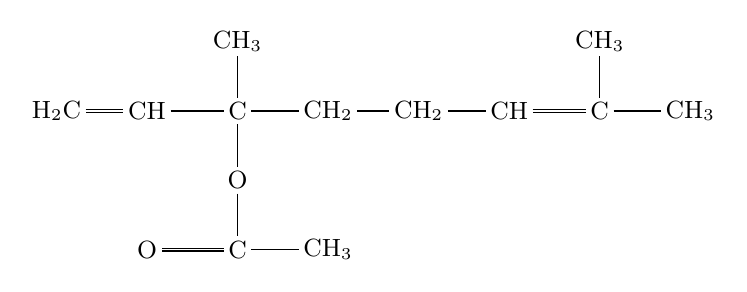
\begin{tikzpicture}[x=1.15cm,y=0.8cm,every node/.style={inner sep=1.5pt,font=\small}]
\node (c1) at (0,0) {H$_2$C};
\node (c2) at (1,0) {CH};
\node (c3) at (2,0) {C};
\node (c4) at (3,0) {CH$_2$};
\node (c5) at (4,0) {CH$_2$};
\node (c6) at (5,0) {CH};
\node (c7) at (6,0) {C};
\node (c8) at (7,0) {CH$_3$};
\node (m3) at (2,1.1) {CH$_3$};
\node (m7) at (6,1.1) {CH$_3$};
\node (o1) at (2,-1.1) {O};
\node (cc) at (2,-2.2) {C};
\node (o2) at (1,-2.2) {O};
\node (ma) at (3,-2.2) {CH$_3$};
\draw[double] (c1) -- (c2);
\draw (c2) -- (c3) (c3) -- (c4) (c4) -- (c5) (c5) -- (c6);
\draw[double] (c6) -- (c7);
\draw (c7) -- (c8) (c3) -- (m3) (c7) -- (m7) (c3) -- (o1) (o1) -- (cc) (cc) -- (ma);
\draw[double] (cc) -- (o2);
\end{tikzpicture}
\end{center}
Em forma condensada: $\mathrm{H_2C{=}CH{-}C(CH_3)(OCOCH_3){-}CH_2{-}CH_2{-}CH{=}C(CH_3){-}CH_3}$.

\textbf{b)} A dupla mais substituída é a $\mathrm{C6{=}C7}$ (trissubstituída, $\mathrm{{-}CH{=}C(CH_3)_2}$). A dupla $\mathrm{C1{=}C2}$ é apenas monossubstituída. Na poliadição, a ligação $\pi$ de $\mathrm{C6{=}C7}$ se abre. A via mais plausível é a catiônica, porque gera um carbocátion terciário em C7. Cada monômero passa a se ligar aos vizinhos por C6 e C7, que formam a cadeia principal do polímero, e o restante da molécula (com o vinil e o acetato intactos) fica como grupo lateral:
\[
n\ \mathrm{CH_2{=}CH{-}C(CH_3)(OCOCH_3){-}CH_2CH_2{-}CH{=}C(CH_3)_2}\ \longrightarrow\ \mathrm{\left[\,CH(R){-}C(CH_3)_2\,\right]_n}
\]
com $\mathrm{R={-}CH_2{-}CH_2{-}C(CH_3)(OCOCH_3){-}CH{=}CH_2}$. Unidade de repetição:
\begin{center}
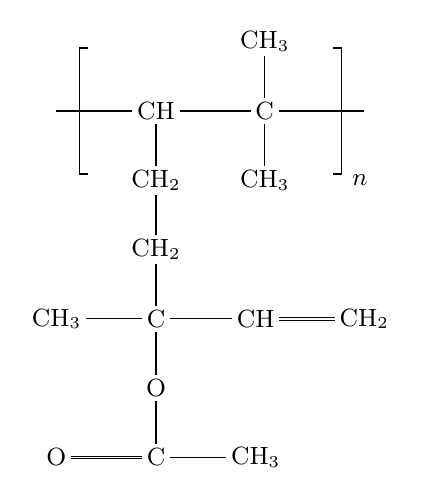
\begin{tikzpicture}[x=1.15cm,y=0.8cm,every node/.style={inner sep=1.5pt,font=\small}]
\node (a) at (0,0) {CH};
\node (b) at (1.2,0) {C};
\node (bm1) at (1.2,1.1) {CH$_3$};
\node (bm2) at (1.2,-1.1) {CH$_3$};
\draw (-1.1,0) -- (a) (a) -- (b) (b) -- (2.3,0) (b) -- (bm1) (b) -- (bm2);
\draw (-0.75,1.0) -- (-0.85,1.0) -- (-0.85,-1.0) -- (-0.75,-1.0);
\draw (1.95,1.0) -- (2.05,1.0) -- (2.05,-1.0) -- (1.95,-1.0);
\node at (2.25,-1.1) {$n$};
\node (r1) at (0,-1.1) {CH$_2$};
\node (r2) at (0,-2.2) {CH$_2$};
\node (r3) at (0,-3.3) {C};
\node (r3m) at (-1.1,-3.3) {CH$_3$};
\node (r4) at (1.1,-3.3) {CH};
\node (r5) at (2.3,-3.3) {CH$_2$};
\node (o1) at (0,-4.4) {O};
\node (cc) at (0,-5.5) {C};
\node (o2) at (-1.1,-5.5) {O};
\node (ma) at (1.1,-5.5) {CH$_3$};
\draw (a) -- (r1) (r1) -- (r2) (r2) -- (r3) (r3) -- (r3m) (r3) -- (r4) (r3) -- (o1) (o1) -- (cc) (cc) -- (ma);
\draw[double] (r4) -- (r5);
\draw[double] (cc) -- (o2);
\end{tikzpicture}
\end{center}
Observação: a unidade de repetição tem a mesma fórmula do monômero, $\mathrm{C_{12}H_{20}O_2}$, como deve ocorrer em qualquer poliadição. Na prática, alquenos trissubstituídos polimerizam com dificuldade por impedimento estérico, daí o ``possivelmente'' do enunciado.

ANSWER: a) $\mathrm{H_2C{=}CH{-}C(CH_3)(OCOCH_3){-}CH_2{-}CH_2{-}CH{=}C(CH_3)_2}$ ($\mathrm{C_{12}H_{20}O_2}$, acetato de 3,7-dimetilocta-1,6-dien-3-ila); b) $\mathrm{\left[\,CH(CH_2CH_2C(CH_3)(OCOCH_3)CH{=}CH_2){-}C(CH_3)_2\,\right]_n}$, poliadição na dupla C6=C7.%
\newpage%
\section*{Questão 4}

\section*{Solução}

\textbf{Hipóteses.} A água inicialmente tem pH $=7$ ($[\mathrm{H^+}]=10^{-7}$ mol/L). O sal do contaminante não altera a acidez do meio, e o volume de ácido adicionado é desprezível frente a $200000$ L (confirmado ao final). O ácido acético ($\mathrm{HAc}$) é um ácido fraco monoprótico com $K_a=2{,}0\times10^{-5}$.

\textbf{Condição mínima.} A precipitação exige pH $\le 4$. Como $[\mathrm{H^+}]$ cresce com a concentração analítica $C$ do ácido, a menor massa corresponde a pH $=4$ exatamente:
\[
[\mathrm{H^+}] = 1{,}0\times10^{-4}\ \text{mol/L}.
\]

\textbf{Equilíbrio.} $\mathrm{CH_3COOH \rightleftharpoons H^+ + CH_3COO^-}$.

Balanço de cargas: $[\mathrm{H^+}]=[\mathrm{Ac^-}]+[\mathrm{OH^-}]$. Como $[\mathrm{OH^-}]=10^{-10}$ mol/L e a contribuição da água ($\le 10^{-7}$ mol/L) são desprezíveis frente a $10^{-4}$ mol/L,
\[
[\mathrm{Ac^-}] \simeq [\mathrm{H^+}] = 1{,}0\times10^{-4}\ \text{mol/L}.
\]
Da constante de ionização:
\[
[\mathrm{HAc}] = \frac{[\mathrm{H^+}][\mathrm{Ac^-}]}{K_a} = \frac{(1{,}0\times10^{-4})^2}{2{,}0\times10^{-5}} = 5{,}0\times10^{-4}\ \text{mol/L}.
\]
Balanço de massa (concentração analítica do ácido):
\[
C = [\mathrm{HAc}]+[\mathrm{Ac^-}] = 5{,}0\times10^{-4}+1{,}0\times10^{-4} = 6{,}0\times10^{-4}\ \text{mol/L}.
\]

\textbf{Observação.} O grau de ionização é $\alpha = \dfrac{1{,}0\times10^{-4}}{6{,}0\times10^{-4}} \simeq 17\,\%$, que não é pequeno. Por isso não se pode usar a aproximação $[\mathrm{H^+}]\simeq\sqrt{K_a C}$: ela daria $C=5{,}0\times10^{-4}$ mol/L, ou seja, 100 mol e cerca de 6,0 kg de ácido, o que subestima a massa necessária.

\textbf{Quantidade de matéria por piscina.}
\[
n = C\,V = 6{,}0\times10^{-4}\ \tfrac{\text{mol}}{\text{L}} \times 2{,}0\times10^{5}\ \text{L} = 120\ \text{mol}.
\]

\textbf{Massa.} Para $\mathrm{CH_3COOH}$ ($\mathrm{C_2H_4O_2}$):
\[
M = 2(12{,}011)+4(1{,}0079)+2(15{,}999) \simeq 60{,}05\ \text{g/mol},
\]
\[
m = n\,M = 120 \times 60{,}05 \simeq 7{,}2\times10^{3}\ \text{g} \simeq 7{,}2\ \text{kg}.
\]

\textbf{Verificação.} O ácido acético puro tem densidade próxima de $1{,}05$ g/mL, então $7{,}2$ kg ocupam cerca de $6{,}9$ L. Isso representa cerca de $0{,}003\,\%$ de $200000$ L, o que confirma que a variação de volume é desprezível. A ordem de grandeza (alguns quilogramas para 200 m$^3$ de água) também é coerente.

\medskip
ANSWER: $m_{\min} \simeq 7{,}2\times10^{3}$ g $\approx 7{,}2$ kg de ácido acético por piscina (120 mol, com $C = 6{,}0\times10^{-4}$ mol/L).%
\newpage%
\section*{Questão 5}

\section*{Solução}

\textbf{1. Reação e hipóteses.} A combustão completa do metano com formação de água líquida é
\[
\mathrm{CH_4(g) + 2\,O_2(g) \longrightarrow CO_2(g) + 2\,H_2O(l)}, \qquad \Delta H_c < 0 .
\]
A pressão constante, o calor trocado é igual à variação de entalpia: $Q_p = \Delta H$. A segunda queima ocorre \emph{nas mesmas condições}, ou seja, é a mesma reação (combustão completa, água líquida, mesma $T$ e mesma $p$). Portanto as duas queimas têm o mesmo $\Delta H_c$ por mol de reação.

Como a entalpia é uma grandeza extensiva, a energia liberada é proporcional ao avanço $\xi$ da reação (em mol):
\[
Q = \xi\,|\Delta H_c| .
\]
Por isso não é preciso conhecer $\Delta H_c$, que não aparece na folha de dados: ele se cancela na razão.

\textbf{2. Avanço de cada queima.}
\[
\xi_1 = \frac{324}{|\Delta H_c|}, \qquad \xi_2 = \frac{81}{|\Delta H_c|}
\quad\Longrightarrow\quad \frac{\xi_1}{\xi_2} = \frac{324}{81} = 4 .
\]

\textbf{3. Quantidades de matéria.} Pela estequiometria, $n_{\mathrm{CH_4}} = \xi$ e $n_{\mathrm{O_2}} = 2\xi$:
\[
n_1(\mathrm{CH_4}) = \xi_1 = 4\,\xi_2, \qquad n_2(\mathrm{O_2}) = 2\,\xi_2 .
\]

\textbf{4. Massas molares (tabela fornecida).}
\[
M_{\mathrm{CH_4}} = 12{,}011 + 4(1{,}0079) = 16{,}043\ \mathrm{g\,mol^{-1}}, \qquad
M_{\mathrm{O_2}} = 2(15{,}999) = 31{,}998\ \mathrm{g\,mol^{-1}} .
\]

\textbf{5. Razão pedida.}
\[
\frac{m_1}{m_2} = \frac{n_1(\mathrm{CH_4})\,M_{\mathrm{CH_4}}}{n_2(\mathrm{O_2})\,M_{\mathrm{O_2}}}
= \frac{4\,\xi_2 \cdot 16{,}043}{2\,\xi_2 \cdot 31{,}998}
= \frac{2 \cdot 16{,}043}{31{,}998}
= \frac{32{,}085}{31{,}998} \approx 1{,}003 .
\]
A razão é adimensional e depende apenas da estequiometria e das massas molares.

\textbf{6. Verificação da ordem de grandeza.} Com o valor tabelado típico $|\Delta H_c| \approx 890\ \mathrm{kJ\,mol^{-1}}$ (usado apenas para conferir), temos $\xi_1 \approx 0{,}364$ mol, logo $m_1 \approx 5{,}84$ g de $\mathrm{CH_4}$. Também $\xi_2 \approx 0{,}091$ mol, logo $n(\mathrm{O_2}) \approx 0{,}182$ mol e $m_2 \approx 5{,}83$ g de $\mathrm{O_2}$. A razão é de fato $\approx 1$.

A interpretação física é a seguinte. A primeira queima tem avanço $4$ vezes maior que a segunda. Por outro lado, para um mesmo avanço, a massa de $\mathrm{O_2}$ consumida é $64/16 \approx 4$ vezes a massa de $\mathrm{CH_4}$. Os dois fatores se compensam, e as massas ficam praticamente iguais.

\[
\boxed{\dfrac{m_1}{m_2} = \dfrac{2M_{\mathrm{CH_4}}}{M_{\mathrm{O_2}}} \approx 1{,}003 \approx 1}
\]

ANSWER: $\dfrac{m_1}{m_2} = \dfrac{2 \cdot 16{,}043}{31{,}998} \approx 1{,}003$, ou seja, $m_1 \approx m_2$ (razão $\approx 1$)%
\newpage%
\section*{Questão 6}

\section*{Solução}

\textbf{1) Massa molar pela densidade do vapor (Lei de Avogadro).}
Na mesma temperatura e pressão, volumes iguais de gases ideais contêm o mesmo número de mols. Como $d = \dfrac{PM}{RT}$, a razão entre as densidades é igual à razão entre as massas molares:
\[
\frac{d_{\text{ácido}}}{d_{\mathrm{H_2}}} = \frac{M_{\text{ácido}}}{M_{\mathrm{H_2}}} = 30
\;\Rightarrow\;
M_{\text{ácido}} = 30 \cdot 2 \cdot 1{,}0079 \approx 60{,}5 \ \text{g/mol} \approx 60 \ \text{g/mol}.
\]

\textbf{2) Número de hidrogênios ionizáveis (neutralização).}
Mols de base gastos:
\[
n_{\mathrm{OH^-}} = n_{\mathrm{NaOH}} = 0{,}1 \ \text{mol/L} \cdot 0{,}030 \ \text{L} = 3{,}0 \times 10^{-3} \ \text{mol}.
\]
Mols de ácido na amostra:
\[
n_{\text{ácido}} = \frac{0{,}18 \ \text{g}}{60 \ \text{g/mol}} = 3{,}0 \times 10^{-3} \ \text{mol}.
\]
Como o ácido se dissocia completamente, cada H ionizável (o H da carboxila) reage com um $\mathrm{OH^-}$, na proporção $1:1$. Seja $x$ o número de grupos $-\mathrm{COOH}$:
\[
x = \frac{n_{\mathrm{OH^-}}}{n_{\text{ácido}}} = \frac{3{,}0 \times 10^{-3}}{3{,}0 \times 10^{-3}} = 1 .
\]
Dito de outro modo, a massa equivalente vale $0{,}18/3{,}0\times 10^{-3} = 60$ g/eq, que é igual a $M/x$. Portanto o ácido é \textbf{monocarboxílico}: $\mathrm{R{-}COOH}$.

\textbf{3) Identificação do radical.}
A carboxila $-\mathrm{COOH}$ tem massa $12 + 2\cdot 16 + 1 = 45$ g/mol. Logo
\[
M_{\mathrm{R}} = 60 - 45 = 15 \ \text{g/mol} \;\Rightarrow\; \mathrm{R} = -\mathrm{CH_3}\quad(12 + 3 \cdot 1 = 15).
\]
Pela fórmula geral dos ácidos monocarboxílicos saturados, $\mathrm{C_nH_{2n}O_2}$, chega-se ao mesmo resultado: $14n + 32 = 60 \Rightarrow n = 2$. Ficam excluídos os vizinhos da série, o ácido fórmico ($M = 46$) e o propanoico ($M = 74$).

\textbf{Verificação:} para $\mathrm{C_2H_4O_2}$, $M = 2(12{,}011) + 4(1{,}0079) + 2(15{,}999) \approx 60{,}05$ g/mol. Então $n = 0{,}18/60{,}05 \approx 3{,}0 \times 10^{-3}$ mol, coerente com
\[
\mathrm{CH_3COOH + NaOH \longrightarrow CH_3COONa + H_2O}.
\]
A diferença entre $60{,}5$ e $60{,}05$ é menor que $1\%$ e cabe na precisão dos dados ($0{,}18$ g tem 2 algarismos significativos). Observação: a densidade dada corresponde ao monômero. Na prática, o vapor de ácido acético tende a formar dímeros, mas o enunciado fixa $M \approx 60$.

\textbf{Resposta.} Ácido \textbf{etanoico} (ácido acético), de fórmula molecular $\mathrm{C_2H_4O_2}$ e fórmula estrutural:
\begin{center}
\begin{tikzpicture}
\node (C1) at (0,0) {$\mathrm{H_3C}$};
\node (C2) at (1.4,0) {$\mathrm{C}$};
\node (O1) at (2.3,0.8) {$\mathrm{O}$};
\node (O2) at (2.3,-0.8) {$\mathrm{O}$};
\node (H) at (3.3,-0.8) {$\mathrm{H}$};
\draw (C1) -- (C2);
\draw[double, double distance=2pt] (C2) -- (O1);
\draw (C2) -- (O2);
\draw (O2) -- (H);
\end{tikzpicture}
\end{center}
isto é, $\mathrm{H_3C{-}C({=}O){-}OH}$.

ANSWER: Ácido etanoico (ácido acético), $\mathrm{CH_3COOH}$ ($\mathrm{C_2H_4O_2}$, $M \approx 60$ g/mol, monoprótico): $\mathrm{H_3C{-}C({=}O){-}OH}$.%
\newpage%
\section*{Questão 7}

\section*{Solução}

\textbf{1) Reação global (Lei de Hess).} Somando as três etapas, sendo a terceira multiplicada por 2, o CuO e o Cu(s) se cancelam:
\[
\text{Cu}_2\text{CO}_3(\text{OH})_2(s) + \text{C}(s,\ \text{grafite}) \longrightarrow 2\,\text{Cu}(l) + \text{H}_2\text{O}(g) + 2\,\text{CO}_2(g).
\]
Pela hipótese (iii), as entalpias de formação não variam entre 298 e 1358 K. Assim, os $\Delta H_f^o$ tabelados a 25 °C valem na temperatura do processo, e a água sai como vapor.

\textbf{2) Etapas 1 e 2 juntas.} O $\Delta H_f^o$ do CuO não é dado, mas ele se cancela na soma. Lembre que $\Delta H_f^o = 0$ para C(grafite) e Cu(s):
\[
\Delta H_{1+2} = \left[2(-394{,}0) + (-242{,}0)\right] - \left[(-1054{,}0) + 0\right] = +24{,}0\ \text{kJ por mol de malaquita}.
\]

\textbf{3) Entalpia de fusão do cobre.} Na temperatura de fusão as duas fases coexistem em equilíbrio, logo $G_S = G_L$. Todos os termos idênticos se cancelam:
\[
G_L - G_S = (5194{,}3 + 7770{,}5) + (120{,}0 - 130{,}0)T = 12964{,}8 - 10{,}0\,T = 0
\;\Longrightarrow\; T_{fus} = 1296{,}48\ \text{K}.
\]
Como no equilíbrio $\Delta G_{fus} = \Delta H_{fus} - T_{fus}\Delta S_{fus} = 0$, usamos o $\Delta S^o_{fus}$ da folha de dados:
\[
\Delta H_{fus} = T_{fus}\,\Delta S_{fus} = 1296{,}48 \times 10{,}0 = 12964{,}8\ \text{J/mol} \approx 12{,}96\ \text{kJ/mol}.
\]
Há uma conferência de unidades. Comparando $G_L - G_S = \Delta H_{fus} - T\Delta S_{fus}$ com a expressão acima, obtém-se $\Delta S_{fus} = -\frac{d(G_L - G_S)}{dT} = 10{,}0$, que coincide com o valor dado apenas se as expressões de $G$ estiverem em J/mol. Em kJ/mol teríamos $\Delta H_{fus} \approx 1{,}3\times 10^{4}\ \text{kJ/mol}$, valor absurdo (o real é cerca de 13 kJ/mol). Portanto o rótulo ``kJ/mol'' do enunciado deve ser lido como J/mol. O caminho por $T_{fus}\Delta S_{fus}$ não depende dessa unidade.

\textbf{4) Entalpia da reação global.}
\[
\Delta H_{global} = 24{,}0 + 2(12{,}96) \approx +49{,}93\ \text{kJ por mol de malaquita} = 24{,}96\ \text{kJ por mol de Cu}(l).
\]
O valor é positivo, ou seja, a reação é endotérmica, como afirma o enunciado.

\textbf{5) Energia para 213,36 kg de Cu.}
\[
n_{\text{Cu}} = \frac{213360\ \text{g}}{63{,}546\ \text{g/mol}} \approx 3{,}358\times 10^{3}\ \text{mol}
\;\Longrightarrow\; n_{\text{malaquita}} = \frac{n_{\text{Cu}}}{2} \approx 1678{,}8\ \text{mol}.
\]
\[
E = 1678{,}8 \times 49{,}93\ \text{kJ} \approx 8{,}38\times 10^{4}\ \text{kJ} \approx 83{,}8\ \text{MJ}.
\]
Com $M \approx 63{,}5$ g/mol, tem-se $n_{\text{Cu}} = 3360$ mol e $E \approx 83{,}9$ MJ, o que não muda o resultado.

\textbf{6) Número de placas.} A energia mínima é o próprio $\Delta H$ do processo a pressão constante, sem perdas. Em 1 h cada placa fornece 2 MJ:
\[
N \ge \frac{83{,}8\ \text{MJ}}{2\ \text{MJ/placa}} \approx 41{,}9.
\]
Como $N$ deve ser inteiro, são necessárias no mínimo $N = 42$ placas.

ANSWER: 42 placas solares ($\Delta H_{global} \approx +49{,}9$ kJ por mol de malaquita; energia $\approx 83{,}8$ MJ em 1 h)%
\newpage%
\section*{Questão 8}

\section*{Solução}

\textbf{Ideia.} Comparamos o número de elétrons de valência que o ânion realmente tem com o número que seria necessário se cada traço da figura (cada par de átomos ligados) fosse uma ligação comum de 2 centros e 2 elétrons (2c--2e).

\medskip
\textbf{1) Elétrons de valência disponíveis em $[\mathrm{B_{12}H_{12}}]^{2-}$.}
O boro (grupo 13) tem 3 elétrons de valência, o hidrogênio tem 1, e a carga $2-$ acrescenta 2 elétrons:
\[
N_{\text{real}} = 12\cdot 3 + 12\cdot 1 + 2 = 36 + 12 + 2 = 50 \text{ elétrons}.
\]

\medskip
\textbf{2) Número de ligações se todas fossem 2c--2e.}
\begin{itemize}
\item \emph{Ligações B--H terminais:} cada vértice é um grupo B--H, logo há $12$ ligações B--H.
\item \emph{Ligações B--B (arestas do icosaedro):} o icosaedro tem $V = 12$ vértices, e em cada vértice chegam 5 arestas (na figura, cada B se liga a 5 outros B). Cada aresta liga dois vértices, então
\[
A = \frac{12\cdot 5}{2} = 30 .
\]
Conferência pela relação de Euler: as 20 faces são triângulos, e $V - A + F = 12 - 30 + 20 = 2$. Está correto.
\end{itemize}
Total de ligações: $30 + 12 = 42$. Como cada ligação comum usa 2 elétrons,
\[
N_{\text{esperado}} = 2\cdot 42 = 84 \text{ elétrons}.
\]

\medskip
\textbf{3) Deficiência percentual.}
\[
\text{Deficiência} = \frac{N_{\text{esperado}} - N_{\text{real}}}{N_{\text{esperado}}}\cdot 100\%
= \frac{84 - 50}{84}\cdot 100\% = \frac{34}{84}\cdot 100\% \approx 40{,}5\% .
\]
Faltam, portanto, 34 elétrons (17 pares).

\medskip
\textbf{Verificações.}
\begin{itemize}
\item \emph{Mesmo critério aplicado ao diborano:} o $\mathrm{B_2H_6}$ tem $2\cdot 3 + 6\cdot 1 = 12$ elétrons. Com ligações comuns, ele teria 4 ligações B--H terminais e 4 ligações B--H em ponte, o que exigiria $8\cdot 2 = 16$ elétrons. A deficiência seria então $4/16 = 25\%$, menor que a do dodecaborato. Isso faz sentido, porque o ânion tem uma estrutura em gaiola muito mais conectada.
\item \emph{Onde está a falta de elétrons:} as 12 ligações B--H terminais são ligações comuns e usam $24$ elétrons. Sobram $50 - 24 = 26$ elétrons, ou seja, 13 pares, para a gaiola de $\mathrm{B_{12}}$. Esse valor é o previsto pela regra de Wade para um \emph{closo}-borano com $n = 12$ vértices ($n+1 = 13$ pares). Com ligações comuns, as 30 arestas exigiriam $60$ elétrons. Os 34 elétrons que faltam estão, portanto, todos na gaiola, que se mantém por ligações deslocalizadas de vários centros, como as ligações de 3 centros e 2 elétrons do diborano.
\end{itemize}

\medskip
ANSWER: O ânion tem $50$ elétrons de valência, mas precisaria de $2\cdot(30+12) = 84$ se todas as ligações fossem comuns (2 centros, 2 elétrons). A deficiência é $\dfrac{34}{84} \approx 40{,}5\%$.%
\newpage%
\section*{Questão 9}

\section*{Solução}

\textbf{a) CO$_2$ dissolvido (lei de Henry).}
Hipóteses: ar como gás ideal à pressão total $P=1$ atm. Pela lei de Dalton, a pressão parcial é a fração molar vezes a pressão total, com $545$ ppm (base molar) $\Rightarrow x_{\mathrm{CO_2}}=545\times10^{-6}$:
\[
p_{\mathrm{CO_2}}=x_{\mathrm{CO_2}}\,P=5{,}45\times10^{-4}\ \text{atm}.
\]
Lei de Henry (solução diluída em equilíbrio com o gás), usando a constante dada ($300\ \text{K}\approx 298\ \text{K}$):
\[
[\mathrm{CO_2(aq)}]=k_H\,p_{\mathrm{CO_2}}=3{,}3\times10^{-2}\cdot5{,}45\times10^{-4}\approx 1{,}8\times10^{-5}\ \text{mol}\cdot\text{L}^{-1}.
\]
Observação: corrigir $k_H$ de 300 K para 298 K com van't Hoff, usando $\Delta H_{dis}=-413{,}8-(-394{,}0)=-19{,}8$ kJ/mol, dá $k_H\approx3{,}5\times10^{-2}$ e $[\mathrm{CO_2}]\approx1{,}9\times10^{-5}$ mol/L. A diferença é de cerca de 5\%, o que muda o pH só em cerca de 0,01.

\textbf{b) pH.}
Equilíbrio dominante: $\mathrm{CO_2(aq)+H_2O(l)\rightleftharpoons H^+(aq)+HCO_3^-(aq)}$.
\[
\Delta G^o=-586{,}8+0-(-386{,}0-237{,}1)=+36{,}3\ \text{kJ}\cdot\text{mol}^{-1}
\]
\[
\ln K_a=-\frac{\Delta G^o}{RT}=-\frac{36300}{8{,}3\cdot298}\approx-14{,}68
\;\Rightarrow\;
\log K_a\approx0{,}434\cdot(-14{,}68)\approx-6{,}37,
\]
ou seja, $K_a\approx4{,}3\times10^{-7}$.

Como a solução está em equilíbrio com a atmosfera, o CO$_2$ consumido na ionização é reposto pelo ar. Assim, $[\mathrm{CO_2(aq)}]=C=1{,}8\times10^{-5}$ mol/L no equilíbrio, sem precisar subtrair $x$.

Desprezamos a 2ª ionização, porque o meio é ácido e o carbonato é desprezível. Desprezamos também a autoionização da água: $K_aC\approx7{,}7\times10^{-12}\gg K_w=10^{-14}$. Então $[\mathrm{H^+}]\approx[\mathrm{HCO_3^-}]$ e
\[
[\mathrm{H^+}]^2=K_a\,C\;\Rightarrow\;\mathrm{pH}=\tfrac12\left(pK_a-\log C\right).
\]
Com $\log 1{,}8=\log2+2\log3-1=0{,}255$, temos $\log C=-4{,}745$. Logo
\[
\mathrm{pH}=\tfrac12\,(6{,}37+4{,}745)\approx 5{,}56 .
\]
Conferência: $[\mathrm{H^+}]\approx2{,}8\times10^{-6}$ mol/L e $[\mathrm{OH^-}]\approx3{,}6\times10^{-9}$ mol/L, de fato desprezível. O resultado é coerente com o pH conhecido da chuva \emph{natural}, $\approx5{,}6$. Se o CO$_2$ fosse tratado como sistema fechado ($C-x$ no denominador), o pH seria $\approx5{,}59$, praticamente igual.

\textbf{c) Efeito da temperatura.}
Entalpia da ionização:
\[
\Delta H^o=-692{,}0+0-(-413{,}8-285{,}8)=+7{,}6\ \text{kJ}\cdot\text{mol}^{-1}>0 .
\]
Pela equação de van't Hoff, $\dfrac{d\ln K_a}{dT}=\dfrac{\Delta H^o}{RT^2}>0$. Como a reação é endotérmica, $K_a$ \emph{aumenta} com $T$ (princípio de Le Chatelier). Com $C$ mantido constante, $[\mathrm{H^+}]=\sqrt{K_aC}$ aumenta e, portanto, o pH \textbf{diminui}.

Ordem de grandeza: de 298 K para 308 K, $\Delta\mathrm{pH}=-\tfrac12\cdot0{,}434\cdot\frac{7600}{8{,}3}\left(\frac1{298}-\frac1{308}\right)\approx-0{,}02$.

ANSWER: a) $[\mathrm{CO_2}]\approx1{,}8\times10^{-5}$ mol/L; b) pH $\approx5{,}56$ ($K_a\approx4{,}3\times10^{-7}$); c) o pH diminui, pois a ionização é endotérmica ($\Delta H^o=+7{,}6$ kJ/mol), então $K_a$ e $[\mathrm{H^+}]$ aumentam com $T$.%
\newpage%
\section*{Questão 10}

\section*{Solução}

\textbf{Identificação dos nuclídeos.} Pelos números atômicos: $Z=89$ (Ac), $90$ (Th), $88$ (Ra), $86$ (Rn), $84$ (Po). Logo, X $=\,^{227}_{89}\text{Ac}$, J $=\,^{227}_{90}\text{Th}$, L $=\,^{223}_{88}\text{Ra}$, Z $=\,^{219}_{86}\text{Rn}$ (actinônio) e T $=\,^{215}_{84}\text{Po}$.

\medskip
\textbf{a)} Em cada etapa impomos a conservação do número de massa $A$ e da carga (número atômico). Uma emissão $\alpha={}^{4}_{2}\text{He}$ faz $\Delta A=-4$ e $\Delta Z=-2$. Uma emissão $\beta^-={}^{0}_{-1}\text{e}$ faz $\Delta A=0$ e $\Delta Z=+1$.
\begin{align*}
{}^{227}_{89}\text{Ac} &\longrightarrow {}^{227}_{90}\text{Th} + {}^{0}_{-1}\beta \quad (\Delta A=0,\ \Delta Z=+1)\\
{}^{227}_{90}\text{Th} &\longrightarrow {}^{223}_{88}\text{Ra} + {}^{4}_{2}\alpha \quad (\Delta A=-4,\ \Delta Z=-2)\\
{}^{223}_{88}\text{Ra} &\longrightarrow {}^{219}_{86}\text{Rn} + {}^{4}_{2}\alpha\\
{}^{219}_{86}\text{Rn} &\longrightarrow {}^{215}_{84}\text{Po} + {}^{4}_{2}\alpha
\end{align*}
Somando as etapas e cancelando os intermediários, obtemos a equação global:
\[
{}^{227}_{89}\text{X} \longrightarrow {}^{215}_{84}\text{T} + 3\,{}^{4}_{2}\alpha + {}^{0}_{-1}\beta .
\]
Verificação: massas $227 = 215 + 3\cdot 4 + 0$; cargas $89 = 84 + 3\cdot 2 - 1$. A equação está balanceada.

\medskip
\textbf{b)} No decaimento $\alpha$, $A$ diminui de 4; no decaimento $\beta$ (e na emissão $\gamma$), $A$ não muda. Portanto, o resto de $A$ na divisão por 4 é invariante ao longo de toda a série. Assim, todos os membros de uma mesma família natural têm a forma $A=4n+k$, com $k$ fixo. Aqui:
\[
227=4\cdot 56+3,\quad 223=4\cdot 55+3,\quad 219=4\cdot 54+3,\quad 215=4\cdot 53+3 .
\]
Todos são do tipo $A=4n+3$. Essa é a \textbf{série do actínio} (urânio-actínio), que se inicia no ${}^{235}_{92}\text{U}$ e termina no isótopo estável ${}^{207}_{82}\text{Pb}$ (também $207=4\cdot 51+3$).

\medskip
\textbf{c)} O decaimento é um processo nuclear de primeira ordem, $N(t)=N_0\,e^{-\lambda t}$. Ele não depende de temperatura, pressão ou estado químico, de modo que as condições CNTP e a atmosfera ambiente não alteram $t_{1/2}$.

Na meia-vida, $N=N_0/2$, o que dá $\lambda=\dfrac{\ln 2}{t_{1/2}}$. Com os dados, $\ln 2=\dfrac{\log 2}{0{,}434}=\dfrac{0{,}301}{0{,}434}\simeq 0{,}693$. Então:
\[
\lambda=\frac{0{,}693}{4\ \text{s}}\simeq 0{,}173\ \text{s}^{-1}\;(\approx 1{,}73\times 10^{-1}\ \text{s}^{-1}).
\]
A vida-média é o tempo médio de existência de um núcleo:
\[
\tau=\frac{1}{N_0}\int_0^{\infty} t\,\lambda N_0 e^{-\lambda t}\,dt=\frac{1}{\lambda}=\frac{t_{1/2}}{\ln 2}=\frac{4\ \text{s}}{0{,}693}\simeq 5{,}77\ \text{s}.
\]
Conferência: $\tau>t_{1/2}$, como deve ocorrer, pois $\tau=t_{1/2}/\ln 2\approx 1{,}44\,t_{1/2}$. As unidades estão no SI (s e s$^{-1}$).

\medskip
ANSWER: a) ${}^{227}_{89}\text{X}\to{}^{215}_{84}\text{T}+3\,{}^{4}_{2}\alpha+{}^{0}_{-1}\beta$ (etapas: $\beta^-$, $\alpha$, $\alpha$, $\alpha$; X = Ac, J = Th, L = Ra, Z = Rn, T = Po). b) Todos os nuclídeos têm $A=4n+3$, logo pertencem à série do actínio (${}^{235}\text{U}\to{}^{207}\text{Pb}$). c) $\lambda\simeq 0{,}173\ \text{s}^{-1}$ e $\tau\simeq 5{,}77\ \text{s}$.%
\newpage%
\section*{Apêndice: parecer do avaliador}%
\subsection*{Questão 1: nota 9,5 (aprovada, rodada 1 de 1)}%
\textbf{Resposta da resolução às cegas do avaliador:} Q = 0,4 $\times$ 6,7 $\times$ 3600 = 9648 C, o que dá n(e$^{-}$) = 9648/96480 = 0,10 mol. Como o metal é M$^2$? (vem de MCl$_{2}$), n(M) = 0,050 mol e a massa molar é 4,38/0,050 = 87,6 g/mol. O metal M é o estrôncio (Sr, Z = 38, grupo 2), e o sal é SrCl$_{2}$.\par %
Conferi o enunciado no PDF original (página 2): o texto bate com a transcrição. As contas também estão certas: Q = 0,4 $\times$ 6,7 $\times$ 3600 = 9648 C; n(e$^{-}$) = 9648/96480 = 0,100 mol; n(M) = 0,050 mol; massa molar = 4,38/0,050 = 87,6 g/mol. Conferi tudo em python. A resposta final, estrôncio (Sr, Z = 38, sal SrCl$_{2}$), coincide com a minha referência e está correta. Testei também as cargas erradas: z = 1 dá 43,8 g/mol e z = 3 dá 131,4 g/mol, nenhum metal coerente com os dados, o que reforça z = 2.\newline%
\newline%
Armadilhas que o candidato tratou:\newline%
{-} Carga M$^2$?, deduzida da neutralidade de MCl$_{2}$.\newline%
{-} Conversão de 6,7 h para 24 120 s.\newline%
{-} Uso de F = 96 480 C/mol, como fornecido, o que deixa a conta exata.\newline%
{-} Semirreações do cátodo e do ânodo no sal fundido.\newline%
{-} Hipóteses de corrente constante e eficiência de corrente de 100\%, declaradas logo no início.\newline%
{-} Comentário de que em solução aquosa a água seria reduzida no lugar do Sr.\newline%
{-} Análise de unidades e ordem de grandeza.\newline%
{-} Verificação de que o Sr pertence ao grupo 2, coerente com MCl$_{2}$.\newline%
\newline%
As falhas são todas menores:\newline%
{-} Rb e Y são descartados só pela massa, sem dizer explicitamente que formariam RbCl e YCl$_{3}$.\newline%
{-} Falta a equação global com os estados físicos.\newline%
{-} A afirmação sobre a obtenção industrial do Sr é imprecisa.\newline%
\newline%
A resolução é limpa, completa e bem justificada, no nível de um gabarito comentado.%
\begin{itemize}%
\item%
{[}minor{]} Os vizinhos Rb (85,47) e Y (88,91) são descartados só pela massa. O critério de valência aparece apenas como verificação posterior do Sr, sem dizer que Rb formaria RbCl e Y formaria YCl$_{3}$. Faltou uma frase explícita usando a valência para eliminar esses dois candidatos, o que deixaria a identificação imune a variações de arredondamento (com t entre 6,65 e 6,75 h, a massa molar varia de 87,0 a 88,3 g/mol).%
\item%
{[}minor{]} As semirreações estão escritas, mas falta a equação global MCl$_{2}$(l) $\to$ M(s) + Cl$_{2}$(g), ou SrCl$_{2}$(l) $\to$ Sr(s) + Cl$_{2}$(g). Também faltam os estados físicos (l) dos íons no meio fundido. O ideal é escrever a reação global da eletrólise ígnea com os estados.%
\item%
{[}minor{]} A frase 'o Sr metálico é obtido justamente por eletrólise do sal fundido' simplifica demais. Hoje a produção industrial usa principalmente a redução aluminotérmica de SrO. A eletrólise de SrCl$_{2}$ fundido (com KCl) é uma via possível, não a única. Seria melhor escrever 'pode ser obtido'. O comentário é lateral e não afeta a resposta.%
\end{itemize}%
\subsection*{Questão 2: nota 9,0 (aprovada, rodada 1 de 1)}%
\textbf{Resposta da resolução às cegas do avaliador:} Fiz a resolução de referência da questão 2 conferindo o enunciado no PDF. Tentei confirmar as fórmulas com RDKit, mas o módulo não está instalado; então contei as fórmulas moleculares e os estereocentros à mão.\newline%
\newline%
a) C é um **álcool**, especificamente um álcool terciário. Por isso não é oxidado pelo KMnO4 em meio ácido.\newline%
\newline%
b)\newline%
{-} **A = 1{-}cloro{-}2{-}metilbutano**, ClCH2--CH(CH3)--CH2CH3. É o único C5H11Cl cuja eliminação só pode dar B. O 2{-}cloro{-}2{-}metilbutano também serve, desde que a resolução justifique a regra de Hofmann com base volumosa.\newline%
{-} **B = 2{-}metilbut{-}1{-}eno**, CH2=C(CH3)--CH2CH3. Na ozonólise dá formaldeído + butanona.\newline%
{-} **C = 2{-}metilbutan{-}2{-}ol**, (CH3)2C(OH)--CH2CH3.\par %
Conferi o enunciado no PDF (página 2) e ele bate com a transcrição. Item por item, as respostas finais do candidato coincidem com as da minha referência. (a) C é um álcool terciário. (b) A = 1{-}cloro{-}2{-}metilbutano, B = 2{-}metilbut{-}1{-}eno e C = 2{-}metilbutan{-}2{-}ol. A ozonólise de B dá HCHO + butanona. Estão corretas.\newline%
\newline%
O raciocínio é completo e bem encadeado. A ozonólise com formaldeído indica dupla terminal. Os três alcenos C5H10 com =CH2 são varridos com hidratação de Markovnikov, e o teste do KMnO4/H+ (álcool terciário, sem H no carbono da hidroxila) descarta os dois que dão álcool secundário. O 2{-}metilbut{-}2{-}eno é descartado porque sua ozonólise dá acetona + acetaldeído. Para A, a escolha é o 1{-}cloro{-}2{-}metilbutano, cujo único carbono $\beta$ com H é o C2, de modo que B é o produto único. O candidato também conta os hidrogênios, aponta o estereocentro e declara a hipótese de não haver rearranjo do carbocátion.\newline%
\newline%
Quase todas as armadilhas foram tratadas. Faltam só ressalvas menores: a equação de eliminação está escrita com '+ HCl' em vez de KCl + H2O, não há menção ao 2{-}cloro{-}2{-}metilbutano com base volumosa (Hofmann) como alternativa aceitável, o cloreto de neopentila não é descartado explicitamente e as consequências do rearranjo não são comentadas. Nenhuma delas compromete a correção. A resolução tem qualidade de gabarito comentado.%
\begin{itemize}%
\item%
{[}minor{]} A equação da eliminação traz KOH/etanol como reagente e '+ HCl' como produto. Com KOH, os produtos corretos são KCl + H2O, ou seja, A + KOH $\to$ B + KCl + H2O. O texto diz que o HCl 'é neutralizado pela base', mas a equação deveria mostrar isso.%
\item%
{[}minor{]} O 2{-}cloro{-}2{-}metilbutano é descartado só pela regra de Zaitsev, sem dizer que com base volumosa (t{-}BuOK, produto de Hofmann) ele também forma o 2{-}metilbut{-}1{-}eno como produto principal. Portanto ele é uma resposta alternativa aceitável. A escolha do candidato, o 1{-}cloro{-}2{-}metilbutano, é a mais rigorosa e está certa. Ainda assim, citar a alternativa protegeria a resolução caso o gabarito oficial use o haleto terciário.%
\item%
{[}minor{]} Os outros isômeros C5H11Cl (1{-}cloro{-}3{-}metilbutano, 2{-}cloro{-}3{-}metilbutano, cloretos de pentila e cloreto de neopentila sem H em carbono $\beta$) não são descartados um a um. O argumento 'esqueleto do 2{-}metilbutano com Cl em C1 ou C2' cobre esses casos de forma implícita e é logicamente suficiente, mas uma frase sobre o cloreto de neopentila deixaria a varredura explícita.%
\item%
{[}minor{]} A hipótese 'Markovnikov sem rearranjo, como é usual' está declarada, mas a resolução não diz o que mudaria com rearranjo. No 3{-}metilbut{-}1{-}eno, um deslocamento 1,2 de hidreto daria o 2{-}metilbutan{-}2{-}ol, e B ficaria ambíguo. Declarar a hipótese basta no nível da prova; o comentário só tornaria a resolução mais completa.%
\end{itemize}%
\subsection*{Questão 3: nota 9,5 (aprovada, rodada 1 de 1)}%
\textbf{Resposta da resolução às cegas do avaliador:} a) O acetato de linalila é C12H20O2: a fórmula mínima C6H10O multiplicada por 2. Estrutura: CH2=CH--C(CH3)(O--C(=O)--CH3)--CH2--CH2--CH=C(CH3)2, ou seja, acetato de 3,7{-}dimetilocta{-}1,6{-}dien{-}3{-}ila. O C3 é quaternário e leva o CH3 e o acetato; o C7 tem duas metilas (C8 e a ramificação).\newline%
b) A dupla que polimeriza é a trissubstituída C6=C7. O polímero é --{[}CH(--CH2--CH2--C(CH3)(OCOCH3)--CH=CH2)--C(CH3)2{]}n--. A cadeia principal é formada por C6 e C7. O vinil (C1=C2) e o grupo acetato ficam como grupos laterais sem reagir.\par %
Conferi a transcrição com a página 2 do PDF original e ela está fiel. As respostas finais do candidato coincidem com a minha referência nos dois itens.\newline%
\newline%
a) CH2=CH--C(CH3)(OCOCH3)--CH2--CH2--CH=C(CH3)2, C12H20O2, acetato de 3,7{-}dimetilocta{-}1,6{-}dien{-}3{-}ila.\newline%
\newline%
b) Poliadição na dupla trissubstituída C6=C7, que dá --{[}CH(CH2CH2C(CH3)(OCOCH3)CH=CH2)--C(CH3)2{]}n--. A cadeia principal é formada por C6 e C7, e o vinil e o acetato ficam pendentes, sem reagir.\newline%
\newline%
Conferências feitas:\newline%
{-} Fórmula molecular: a fórmula mínima C6H10O foi dobrada para C12H20O2 por causa dos 2 O.\newline%
{-} Insaturações: IDH = 3, isto é, 2 C=C e 1 C=O, sem anel.\newline%
{-} Massa molar: 196,29 g/mol.\newline%
{-} Hidrogênios: a contagem dá 20.\newline%
{-} Resto alquenila: C10H17.\newline%
{-} Carbono do item v: o candidato identifica os alílicos não terminais (C3 e C5) e escolhe C3, vizinho do vinil monossubstituído. Isso está correto e foi justificado.\newline%
{-} Acetato: escrito corretamente como éster ligado pelo O (R--O--CO--CH3).\newline%
{-} Desenhos: compilei os dois TikZ. Eles renderizam corretamente, com as duplas C=C e C=O visíveis, os colchetes cortando apenas as ligações da cadeia principal e o índice n.\newline%
\newline%
Armadilhas que o candidato tratou:\newline%
{-} dobrar a fórmula mínima;\newline%
{-} contar os 2 C do acetato;\newline%
{-} a ligação do acetato pelo O;\newline%
{-} a escolha de C3 em vez de C5 ou C4;\newline%
{-} a não conjugação das duplas;\newline%
{-} a escolha da dupla mais substituída;\newline%
{-} os grupos pendentes intactos no polímero;\newline%
{-} a unidade repetitiva com a mesma composição do monômero.\newline%
\newline%
Restam só detalhes de notação e de completude:\newline%
{-} faltam os traços nas pontas da unidade repetitiva na forma linear;\newline%
{-} a justificativa do item iv poderia ser mais explícita sobre C8;\newline%
{-} o encadeamento cabeça{-}cauda não é dito expressamente.\newline%
\newline%
É uma resolução com qualidade de gabarito comentado.%
\begin{itemize}%
\item%
{[}minor{]} Na equação do item b e no ANSWER, a unidade repetitiva {[}CH(R)--C(CH3)2{]}n aparece sem os traços de ligação nas pontas (--{[} ... {]}n--), que mostram a continuação da cadeia. O desenho em TikZ está correto nesse ponto, mas a notação linear deveria ser --{[}CH(R)--C(CH3)2{]}n--.%
\item%
{[}minor{]} Item iv: a resolução afasta a metila em C1, mas não diz por que as metilas não podem estar em C8 (uma metila ali também alongaria a cadeia principal). Também não esclarece que 'duas metilas' quer dizer o próprio C8 terminal mais a ramificação em C7. A frase 'só podem estar em C7' fica um pouco solta. Bastava uma linha a mais.%
\item%
{[}minor{]} O item b não diz com todas as letras que o encadeamento é cabeça{-}cauda (\ldots{}CH(R)--C(CH3)2--CH(R)--C(CH3)2\ldots{}). Isso fica implícito na unidade repetitiva e na menção ao carbocátion terciário em C7 (Markovnikov). O comentário de que o 'possivelmente' do enunciado vem da dificuldade estérica é especulação sem prejuízo.%
\end{itemize}%
\subsection*{Questão 4: nota 9,5 (aprovada, rodada 1 de 1)}%
\textbf{Resposta da resolução às cegas do avaliador:} Para atingir pH = 4, é preciso {[}H?{]} = 10$^{-}$$^{4}$ mol/L. Assim, C(HAc) = x + x$^2$/Ka = 10$^{-}$$^{4}$ + 5 $\times$ 10$^{-}$$^{4}$ = 6,0 $\times$ 10$^{-}$$^{4}$ mol/L. Em 200.000 L, isso dá n = 120 mol. Com M = 60,05 g/mol, a massa mínima é m $\approx$ 7,2 $\times$ 10$^3$ g $\approx$ 7,2 kg de ácido acético por piscina.\newline%
\newline%
Usando a aproximação C - x $\approx$ C, o resultado seria 6,0 kg, que está incorreto por falta de ácido.\par %
Conferi o enunciado no PDF original, página 2, e a transcrição está fiel. A resposta final do candidato coincide com a da referência: C = 6,0$\times$10$^{-}$$^{4}$ mol/L, n = 120 mol e m $\approx$ 7,2$\times$10$^3$ g $\approx$ 7,2 kg de ácido acético por piscina. Refiz todas as contas em python3: C = x + x$^2$/Ka = 6$\times$10$^{-}$$^{4}$; n = 120 mol; M = 60,05 g/mol; m = 7206 g. Na verificação de volume, 6,86 L correspondem a 0,0034 \% de 200.000 L. Também conferi que, com a aproximação indevida, o pH fica em 4,04.\newline%
\newline%
A resolução está bem estruturada:\newline%
{-} Justifica por que a quantidade mínima corresponde a pH = 4 exatamente: {[}H?{]} cresce com C.\newline%
{-} Usa o balanço de cargas para obter {[}Ac$^{-}${]} $\approx$ {[}H?{]}, justificando a aproximação com {[}OH$^{-}${]} = 10$^{-}$$^{1}$$^{0}$.\newline%
{-} Calcula {[}HAc{]} a partir de Ka e soma {[}Ac$^{-}${]} no balanço de massa para obter a concentração analítica. Assim distingue corretamente C, {[}HAc{]} e {[}H?{]}.\newline%
{-} Calcula $\alpha$ $\approx$ 17 \% e explica por que a aproximação $\surd$(KaC) falharia, que é a principal armadilha da questão.\newline%
{-} Converte para mols e massa com a massa molar correta do CH$_{3}$COOH e verifica que o volume de ácido adicionado é desprezível.\newline%
\newline%
Todas as armadilhas foram tratadas: a aproximação indevida, o pH limite, C versus {[}H?{]}, o volume de 2$\times$10$^{5}$ L, a massa molar, Ka tomado como Ka (e não como pKa ou Kb), o volume desprezível e a hidrólise do sal.\newline%
\newline%
Só há ressalvas menores de completude e redação: não quantificou o pH de 4,04 que resultaria da aproximação errada, faltam algumas hipóteses implícitas (temperatura, atividades, efeito da precipitação sobre o H?) e uma frase do balanço de cargas mistura dois argumentos. Nenhuma delas afeta a correção. O nível é de gabarito comentado publicável.%
\begin{itemize}%
\item%
{[}minor{]} A resolução diz que a aproximação C - x $\approx$ C 'subestima a massa necessária', mas não quantifica a consequência. Com 6,0 kg (C = 5$\times$10$^{-}$$^{4}$ mol/L), o pH final seria $\approx$ 4,04 > 4 e o metal não precipitaria. Mostrar esse número deixaria claro que o erro viola a condição do problema, e não apenas a precisão da conta.%
\item%
{[}minor{]} Faltam algumas hipóteses implícitas: Ka válido na temperatura do processo (25 $^\circ$C), uso de concentrações no lugar de atividades, e o fato de a própria reação de precipitação não consumir nem liberar H? de forma relevante. São hipóteses{-}padrão e aceitáveis, mas um gabarito comentado as citaria em uma linha.%
\item%
{[}minor{]} No balanço de cargas, a frase '{[}OH$^{-}${]} = 10$^{-}$$^{1}$$^{0}$ mol/L e a contribuição da água ($\leq$ 10$^{-}$$^{7}$ mol/L) são desprezíveis' mistura dois argumentos: o OH$^{-}$ no equilíbrio e a neutralização da alcalinidade inicial da água neutra (10$^{-}$$^{7}$ mol/L). Ficaria mais claro dizer separadamente que o H? gasto para neutralizar o OH$^{-}$ inicial, cerca de 10$^{-}$$^{7}$ mol/L, é desprezível frente a 10$^{-}$$^{4}$ mol/L. A conclusão está certa.%
\end{itemize}%
\subsection*{Questão 5: nota 9,5 (aprovada, rodada 1 de 1)}%
\textbf{Resposta da resolução às cegas do avaliador:} m$_{1}$/m$_{2}$ = 2$\cdot$M(CH$_{4}$)/M(O$_{2}$) = 2(16,043)/31,998 $\approx$ 1,003 $\approx$ 1. Com M(CH$_{4}$) = 16 e M(O$_{2}$) = 32, a razão é exatamente 1 (m$_{1}$ = m$_{2}$). Fundamento: CH$_{4}$ + 2O$_{2}$ $\to$ CO$_{2}$ + 2H$_{2}$O(l). Como o calor liberado é proporcional ao avanço da reação, n(CH$_{4}$)$_{1}$ = 4$\xi$$_{2}$ e n(O$_{2}$)$_{2}$ = 2$\xi$$_{2}$.\par %
O enunciado foi conferido na página 3 do PDF e confere com a transcrição. A resposta final do candidato, m$_{1}$/m$_{2}$ = 2M(CH$_{4}$)/M(O$_{2}$) $\approx$ 1,003 $\approx$ 1, coincide com a minha referência e está correta. Refiz as contas em Python: com as massas da tabela, a razão dá 1,00273, e o resultado não depende do valor de $\Delta$H\_c usado.\newline%
\newline%
O raciocínio está completo e bem fundamentado:\newline%
{-} escreve a reação balanceada com água líquida;\newline%
{-} justifica que a pressão constante faz o calor corresponder a $\Delta$H;\newline%
{-} interpreta "nas mesmas condições" como a mesma reação, o que garante o mesmo $\Delta$H\_c nas duas queimas;\newline%
{-} usa o avanço $\xi$ e a extensividade da entalpia para mostrar que $\Delta$H\_c se cancela, o que explica por que a folha de dados não traz $\Delta$H\_f(CH$_{4}$).\newline%
\newline%
O candidato tratou todas as armadilhas:\newline%
{-} usou o fator 2 do O$_{2}$;\newline%
{-} tomou M(O$_{2}$) = 31,998, e não a massa do O atômico;\newline%
{-} não inverteu a razão das energias (324/81 = 4);\newline%
{-} deixou claro que o valor de 890 kJ/mol serve só para conferir;\newline%
{-} considerou o O$_{2}$ consumido;\newline%
{-} apresentou tanto 1,003 quanto $\approx$ 1 no arredondamento.\newline%
\newline%
A interpretação física (fator 4 do avanço compensado pelo fator 64/16 das massas) é correta e ajuda a entender o resultado.\newline%
\newline%
Os problemas são só de detalhe: m$_{2}$ $\approx$ 5,82 g e não 5,83 g na conferência numérica, a convenção de sinal de Q\_p poderia ser mais explícita, e há uma inconsistência trivial entre 32,085 e 32,086. A resolução tem qualidade de gabarito comentado.%
\begin{itemize}%
\item%
{[}minor{]} Na verificação numérica (item 6), m$_{2}$ = 0,18202 mol $\times$ 31,998 g/mol = 5,824 g, que arredonda para 5,82 g, e não 5,83 g. Não afeta a conclusão (a razão continua 1,0027). Basta corrigir para m$_{2}$ $\approx$ 5,82 g.%
\item%
{[}minor{]} Convenção de sinal frouxa: o candidato escreve Q\_p = $\Delta$H e logo depois usa Q = $\xi$|$\Delta$H\_c| para a energia liberada. O certo é dizer que o calor recebido pelo sistema é Q\_p = $\Delta$H < 0, de modo que a energia liberada vale -$\Delta$H = $\xi$|$\Delta$H\_c|. Não gera erro, mas o texto deveria deixar o sinal explícito.%
\item%
{[}minor{]} Detalhe de arredondamento: 2 $\times$ 16,043 = 32,086. O candidato escreveu 32,085 porque usou o valor não arredondado 2 $\times$ 16,0426. A diferença é irrelevante, mas a passagem fica inconsistente com o valor 16,043 escrito logo antes.%
\end{itemize}%
\subsection*{Questão 6: nota 9,0 (aprovada, rodada 1 de 1)}%
\textbf{Resposta da resolução às cegas do avaliador:} Pela densidade do vapor, M = 30 $\times$ M(H$_{2}$) = 30 $\times$ 2 $\approx$ 60 g/mol. A base gasta é n(NaOH) = 0,030 $\times$ 0,1 = 3,0 $\times$ 10$^{-}$$^3$ mol, e a massa equivalente é 0,18/0,003 = 60 g por mol de H?. Logo o ácido tem 1 H ionizável (monocarboxílico). Assim, R--COOH com R = 60 - 45 = 15, ou seja, CH$_{3}$. O ácido é o **ácido etanoico (ácido acético)**, CH$_{3}$--COOH (C$_{2}$H$_{4}$O$_{2}$). Estrutura: H$_{3}$C--C(=O)--OH, com o C da carboxila sp$^2$ trigonal plano ligado a um O por dupla ligação e a um grupo OH.\par %
Conferi o enunciado na p. 3 da prova e a transcrição está correta. A resposta final do candidato, ácido etanoico (acético), CH$_{3}$COOH, C$_{2}$H$_{4}$O$_{2}$, H$_{3}$C--C(=O)--OH, coincide com a minha referência e está correta. Refiz as contas em Python: 30$\cdot$2$\cdot$1,0079 = 60,47; M(C$_{2}$H$_{4}$O$_{2}$) = 60,05; n(NaOH) = 3,0$\times$10$^{-}$$^3$ mol; massa equivalente = 60 g/eq; n(ácido) = 2,997$\times$10$^{-}$$^3$ mol. Tudo confere.\newline%
\newline%
Situação de cada armadilha:\newline%
{-} Densidade relativa: o candidato usa M(H$_{2}$) = 2 e não confunde com H.\newline%
{-} Volume: converte 30 mL para 0,030 L corretamente.\newline%
{-} Número de H ionizáveis: determina k = 1 cruzando titulação e massa molar, e ainda apresenta a massa equivalente.\newline%
{-} Precisão de 60,5 contra 60,05: discute explicitamente.\newline%
{-} Homólogos fórmico e propanoico: exclui os dois.\newline%
{-} Nome e estrutura: dá o nome IUPAC e o usual, com estrutura mostrando C=O e O--H.\newline%
{-} H da metila: indica que só o H da carboxila é ionizável.\newline%
{-} Dímeros no vapor: comenta.\newline%
\newline%
Falhas, todas menores:\newline%
{-} Não comenta que o ácido acético é fraco, apesar da hipótese de dissociação completa.\newline%
{-} Não discute os isômeros não ácidos de C$_{2}$H$_{4}$O$_{2}$ nem exclui explicitamente um diprótico.\newline%
{-} A estrutura é semicondensada e sem comentário de geometria.\newline%
{-} O arredondamento 60,5 $\to$ 60 só é justificado no fim.\newline%
\newline%
Nota 9: a resolução é correta, rigorosa e clara, praticamente pronta para gabarito comentado.%
\begin{itemize}%
\item%
{[}minor{]} A hipótese de 'dissociação completa' só é usada para justificar que cada H ionizável consome um OH$^{-}$. O candidato não comenta que o ácido acético é, na verdade, fraco (Ka $\approx$ 1,8$\times$10$^{-}$$^{5}$) nem que a titulação com base forte é quantitativa de qualquer modo. Um gabarito comentado deveria deixar claro que a hipótese é uma idealização do enunciado e não uma propriedade real do ácido identificado.%
\item%
{[}minor{]} A unicidade é tratada apenas dentro da série saturada C?H$_{2}$?O$_{2}$, excluindo o fórmico (46) e o propanoico (74). Faltou dizer que os outros isômeros de C$_{2}$H$_{4}$O$_{2}$ (metanoato de metila, que é éster, e hidroxietanal, que é aldeído/álcool) não são ácidos carboxílicos, e que um diprótico (oxálico, 90) ou um k=2 com M=120 contradizem a densidade do vapor. O argumento x = n(OH$^{-}$)/n(ácido) = 1 já basta logicamente, mas não há exclusão explícita.%
\item%
{[}minor{]} A estrutura foi desenhada de forma semicondensada (H$_{3}$C--C(=O)--OH), sem mostrar as ligações C--H da metila. Isso é aceitável, mas a fórmula estrutural plena seria mais completa para 'estrutura molecular'. Também faltou mencionar, ainda que brevemente, a geometria: C da carboxila sp$^2$ trigonal plano e C da metila sp$^3$ tetraédrico.%
\item%
{[}minor{]} O candidato passa de 60,5 para 60 já no passo 1 ('$\approx$ 60,5 $\approx$ 60') e só justifica o arredondamento no fim, na verificação. Seria mais limpo justificar ali mesmo, ou usar M(H$_{2}$) $\approx$ 2 desde o início. Não há erro numérico: a diferença para 60,05 é de 0,7\%.%
\end{itemize}%
\subsection*{Questão 7: nota 9,5 (aprovada, rodada 1 de 1)}%
\textbf{Resposta da resolução às cegas do avaliador:} {-} Reação global: Cu$_{2}$CO$_{3}$(OH)$_{2}$(s) + C(s) $\to$ 2Cu(l) + H$_{2}$O(g) + 2CO$_{2}$(g)\newline%
{-} $\Delta$H até Cu(s): +24,0 kJ/mol\newline%
{-} T\_fus = 1296,48 K (de G\_S = G\_L) e $\Delta$H\_fus = T\_fus$\cdot$$\Delta$S\_fus $\approx$ 12,96 kJ/mol\newline%
{-} $\Delta$H\_global $\approx$ +49,93 kJ por mol de malaquita\newline%
{-} n(Cu) $\approx$ 3358 mol (3360 com M = 63,5), logo n(malaquita) $\approx$ 1679 mol (1680)\newline%
{-} Energia $\approx$ 83,8--83,9 MJ, o que dá N $\approx$ 41,9\newline%
\newline%
**Mínimo de 42 placas solares.**\par %
Conferi a transcrição com a página 3 da prova original e ela está fiel, inclusive com o anômalo '-2,7$\times$10$^2$' e o rótulo 'kJ/mol'. A resolução do candidato coincide com a minha referência em todos os itens, e a resposta final é a mesma: 42 placas.\newline%
\newline%
Itens conferidos:\newline%
{-} **Reação global (Hess, etapa 3 $\times$2):** Cu$_{2}$CO$_{3}$(OH)$_{2}$ + C $\to$ 2Cu(l) + H$_{2}$O(g) + 2CO$_{2}$(g). O CuO se cancela, e o candidato observa isso.\newline%
{-} **$\Delta$H químico:** +24,0 kJ/mol, com H$_{2}$O(g) e CO$_{2}$(g). Ele evitou corretamente os dados de H$_{2}$O(l) e de CO$_{2}$(aq).\newline%
{-} **Temperatura de fusão:** G\_S = G\_L dá T\_fus = 1296,48 K, dentro da faixa 298--1358 K.\newline%
{-} **$\Delta$H\_fus:** T\_fus$\cdot$$\Delta$S\_fus = 12,96 kJ/mol. A conferência de unidades está correta: -d($\Delta$G)/dT = 10 só é coerente com o $\Delta$S\_fus da folha se G estiver em J/mol, e em kJ/mol daria um valor absurdo de 1,3$\times$10$^{4}$ kJ/mol. O candidato também nota que o caminho T$\cdot$$\Delta$S não depende dessa unidade.\newline%
{-} **$\Delta$H global:** +49,93 kJ por mol de malaquita, coerente com o 'endotérmica' do enunciado.\newline%
{-} **Quantidade de cobre:** n(Cu) = 3357,6 mol, ou 3360 com M = 63,5, e n(malaquita) = 1678,8 mol.\newline%
{-} **Energia:** E $\approx$ 83,8 MJ (83,9 com M = 63,5). Recalculei em python: 83 821 kJ, o que dá 41,91 placas (41,94 com 63,5).\newline%
{-} **Arredondamento:** para cima, 42, justificado pelo caráter de mínimo, com aproveitamento ideal e N inteiro.\newline%
\newline%
Todas as armadilhas listadas foram tratadas: Hess, fase da água, inclusão da fusão de 2 mol de Cu, typo de unidade, não usar $\Delta$G a 298 K, hipótese iii, estequiometria e arredondamento para cima.\newline%
\newline%
Restam apenas detalhes menores:\newline%
{-} 2(12,96) foi somado como 49,93 em vez de 49,92;\newline%
{-} a justificativa do vapor está atribuída à hipótese iii, quando vem da própria equação;\newline%
{-} falta uma menção explícita de que se despreza o calor sensível.\newline%
\newline%
A redação é clara e rigorosa, adequada a gabarito comentado.%
\begin{itemize}%
\item%
{[}minor{]} Inconsistência de arredondamento no passo 4. O texto escreve '24,0 + 2(12,96) $\approx$ +49,93', mas 24,0 + 25,92 = 49,92. O valor 49,93 vem de 12,9648 sem arredondar. Não altera nada (41,9 placas, logo 42), mas deveria escrever 2(12,9648) ou manter 49,92.%
\item%
{[}minor{]} Pequeno non sequitur no passo 1: 'Pela hipótese (iii)... Assim... a água sai como vapor'. O estado da água (g) vem da própria equação da etapa 1 (e da alta temperatura), não da hipótese iii. Bastaria separar as duas justificativas.%
\item%
{[}minor{]} Não diz explicitamente que se despreza o calor sensível para aquecer os reagentes de 298 K até cerca de 1296 K. A hipótese iii e a falta de dados de Cp autorizam isso, e é a leitura pretendida, mas uma frase deixaria claro que 'energia mínima = $\Delta$H da reação global', sem aquecimento e sem perdas. A frase do passo 6 cobre isso só em parte.%
\end{itemize}%
\subsection*{Questão 8: nota 9,3 (aprovada, rodada 1 de 1)}%
\textbf{Resposta da resolução às cegas do avaliador:} O ânion tem 12$\cdot$3 + 12$\cdot$1 + 2 = 50 elétrons de valência. Com só ligações 2c{-}2e, seriam 30 arestas B--B mais 12 ligações B--H, ou seja, 42 ligações e 84 elétrons. A deficiência é (84 - 50)/84 = 34/84 $\approx$ **40,5\%**: o ânion tem cerca de 59,5\% dos elétrons esperados.\par %
Conferi o enunciado na página 4 do PDF e a transcrição está fiel. O candidato chega ao mesmo resultado da minha referência: N\_real = 12$\cdot$3 + 12$\cdot$1 + 2 = 50 elétrons e N\_esperado = 2$\cdot$(30 + 12) = 84 elétrons. A deficiência é 34/84 $\approx$ 40,5\%, calculada sobre o valor esperado, como o enunciado pede. Conferi as contas em python: 40,476\% e 25\% no B2H6.\newline%
\newline%
Todas as armadilhas principais foram tratadas:\newline%
{-} os 2 elétrons da carga 2- entraram na conta;\newline%
{-} as 30 arestas foram contadas certo (12$\cdot$5/2) e conferidas por Euler (12 - 30 + 20 = 2);\newline%
{-} as 12 ligações B--H terminais entraram no total esperado;\newline%
{-} a base da porcentagem é a correta (84, e não 50);\newline%
{-} a resposta dá a deficiência, e não a fração presente de 59,5\%;\newline%
{-} o B tem 3 elétrons de valência;\newline%
{-} a resolução não comparou só o esqueleto, e mesmo assim fez a análise do esqueleto corretamente: 26 elétrons, 13 pares, n + 1 pela regra de Wade para closo{-}borano, e 60 - 26 = 34 elétrons faltando, todos na gaiola.\newline%
\newline%
Há ainda uma boa verificação análoga no B2H6 (16 elétrons esperados contra 12 reais, 25\%). A exposição é clara, organizada e tem rigor suficiente.\newline%
\newline%
Faltou apenas um comentário conceitual: o modelo 2c{-}2e é hipotético, porque exigiria 12 elétrons em volta de cada B, e a referência não é o octeto. Há também pequenas imprecisões de redação. A resolução fica em nível de gabarito comentado publicável, com ressalvas mínimas.%
\begin{itemize}%
\item%
{[}minor{]} A resolução não diz que o modelo só com ligações 2c{-}2e é hipotético. Ele poria 6 ligações, ou seja, 12 elétrons, em volta de cada B, que só tem 4 orbitais de valência (2s, 2p). Também não descarta por que não se usa o octeto como referência, com B tetravalente: 30 ligações, 60 elétrons e cerca de 16,7\%. Basta uma frase dizendo que a referência é a conectividade da figura (5 vizinhos B e 1 H por B) e que esse modelo é impossível, e por isso há ligações multicêntricas. Isso deixaria a escolha do 'esperado' blindada contra uma leitura alternativa.%
\item%
{[}minor{]} A comparação com o B2H6 termina com a frase 'Isso faz sentido, porque o ânion tem uma estrutura em gaiola muito mais conectada'. É só uma justificativa qualitativa, sem peso de verificação. Seria mais limpo apresentar o cálculo do B2H6 apenas como validação do método: o mesmo critério dá 16 elétrons esperados contra 12 reais.%
\item%
{[}minor{]} A resolução diz 'cada traço da figura (cada par de átomos ligados)', mas na figura as ligações B--H terminais aparecem como os rótulos 'HB'/'BH', sem traço. A conclusão de que são 12 ligações B--H está certa. Só a frase de motivação é um pouco imprecisa.%
\end{itemize}%
\subsection*{Questão 9: nota 9,5 (aprovada, rodada 1 de 1)}%
\textbf{Resposta da resolução às cegas do avaliador:} a) {[}CO2(aq){]} = K\_H$\cdot$p(CO2) = 3,3$\times$10$^{-}$$^2$ $\times$ 5,45$\times$10$^{-}$$^{4}$ $\approx$ 1,8$\times$10$^{-}$$^{5}$ mol/L (com p = 545$\times$10$^{-}$$^{6}$ $\times$ 1 atm; se K\_H for corrigido para 298 K, dá $\approx$ 1,9$\times$10$^{-}$$^{5}$ M, também aceitável).\newline%
b) Para CO2(aq) + H2O ? H? + HCO3$^{-}$: $\Delta$G$^\circ$ = +36,3 kJ/mol $\Rightarrow$ log K1 $\approx$ -6,37 (K1 $\approx$ 4,3$\times$10$^{-}$$^{7}$); {[}H?{]} = $\surd$(K1$\cdot${[}CO2{]}) $\approx$ 2,8$\times$10$^{-}$$^{6}$ M $\Rightarrow$ pH $\approx$ 5,56 (faixa aceitável $\approx$ 5,5--5,6).\newline%
c) O pH DIMINUI: a ionização é endotérmica ($\Delta$H$^\circ$ = +7,6 kJ/mol), então K1 aumenta com T (van't Hoff); com {[}CO2(aq){]} fixa, {[}H?{]} = $\surd$(K1{[}CO2{]}) aumenta.\par %
Conferi o enunciado na página 4 do PDF, e a transcrição está fiel. As três respostas finais do candidato coincidem com a minha referência e estão corretas. a) {[}CO2{]} = 3,3$\times$10$^{-}$$^2$ $\times$ 5,45$\times$10$^{-}$$^{4}$ = 1,7985$\times$10$^{-}$$^{5}$ $\approx$ 1,8$\times$10$^{-}$$^{5}$ mol/L. b) $\Delta$G$^\circ$ = +36,3 kJ/mol, ln K = -14,68, log K = -6,37 e pH = $\frac12$(6,37 + 4,745) = 5,557 $\approx$ 5,56. c) $\Delta$H$^\circ$ = +7,6 kJ/mol, logo o pH diminui. Refiz em python os valores secundários e todos batem: correção de k\_H para 298 K = 3,48$\times$10$^{-}$$^2$, o que dá {[}CO2{]} $\approx$ 1,90$\times$10$^{-}$$^{5}$ e $\Delta$pH $\approx$ 0,012; sistema fechado dá pH = 5,591; {[}OH$^{-}${]} = 3,6$\times$10$^{-}$$^{9}$; K\_a$\cdot$C = 7,7$\times$10$^{-}$$^{1}$$^2$ ? K\_w; $\Delta$pH de 298 para 308 K = -0,022; log 1,8 = 0,255.\newline%
\newline%
Todas as armadilhas foram tratadas:\newline%
{-} ppm em base molar foi lido como fração molar, com P = 1 atm declarado.\newline%
{-} A lei de Henry foi aplicada no sentido certo (C = k\_H$\cdot$p), coerente com as unidades.\newline%
{-} A aproximação 300 K $\approx$ 298 K foi explicitada, com uma correção opcional por van't Hoff correta.\newline%
{-} K\_a saiu dos $\Delta$Gf$^\circ$ com T = 298 K e sinal correto.\newline%
{-} O sistema aberto foi tratado corretamente: {[}CO2{]} é a concentração de equilíbrio e não se subtrai x. A variante de sistema fechado aparece como comparação.\newline%
{-} O desprezo da autoionização foi justificado pelo critério certo (K\_aC ? K\_w) e conferido a posteriori.\newline%
{-} No item c, o $\Delta$H$^\circ$ foi calculado a partir dos $\Delta$Hf$^\circ$, e a cadeia de raciocínio está completa: van't Hoff $\to$ K\_a aumenta $\to$ {[}H?{]} = $\surd$(K\_aC) aumenta $\to$ pH diminui. O candidato não caiu na armadilha da solubilidade nem na do $\Delta$S$^\circ$ < 0.\newline%
\newline%
Restam só deslizes formais de rigor:\newline%
{-} a 2ª ionização foi descartada de forma qualitativa e sem citar a eletroneutralidade;\newline%
{-} não foi declarado que $\Delta$H$^\circ$ é suposto constante na van't Hoff integrada;\newline%
{-} o arredondamento de K\_a ficou um pouco generoso.\newline%
\newline%
A resolução tem nível de gabarito comentado.%
\begin{itemize}%
\item%
{[}minor{]} A 2ª ionização (formação de CO3$^2$$^{-}$) é descartada só com o argumento qualitativo de que o meio é ácido. Como a folha de dados não dá Ka2, isso é aceitável, mas faltou dizer que {[}CO3$^2$$^{-}${]} $\approx$ Ka2 \textasciitilde{} 10$^{-}$$^{1}$$^{1}$ M (ordem de grandeza da literatura) é desprezível frente a {[}HCO3$^{-}${]} \textasciitilde{} 10$^{-}$$^{6}$ M. Também faltou citar a eletroneutralidade ({[}H?{]} = {[}HCO3$^{-}${]} + {[}OH$^{-}${]} + 2{[}CO3$^2$$^{-}${]}) como origem de {[}H?{]} $\approx$ {[}HCO3$^{-}${]}.%
\item%
{[}minor{]} Na estimativa de $\Delta$pH entre 298 K e 308 K (item c) e na correção de k\_H entre 300 K e 298 K (item a), a van't Hoff integrada é usada sem declarar que $\Delta$H$^\circ$ foi suposto constante na faixa. A hipótese é óbvia para $\Delta$T de 2 a 10 K, mas um gabarito comentado a deixaria explícita.%
\item%
{[}minor{]} K\_a $\approx$ 4,3$\times$10$^{-}$$^{7}$ é um arredondamento um pouco generoso: exp(-14,676) = 4,23$\times$10$^{-}$$^{7}$ e 10\^{}(-6,37) = 4,27$\times$10$^{-}$$^{7}$. O pH final (5,56) não muda, porque o cálculo segue por pK\_a = 6,37.%
\end{itemize}%
\subsection*{Questão 10: nota 9,5 (aprovada, rodada 1 de 1)}%
\textbf{Resposta da resolução às cegas do avaliador:} a) A série é $^2$$^2$$^{7}$$_{8}$$_{9}$Ac $\to$ $^2$$^2$$^{7}$$_{9}$$_{0}$Th $\to$ $^2$$^2$$^3$$_{8}$$_{8}$Ra $\to$ $^2$$^{1}$$^{9}$$_{8}$$_{6}$Rn $\to$ $^2$$^{1}$$^{5}$$_{8}$$_{4}$Po. A primeira etapa é uma emissão $\beta$$^{-}$ e as três seguintes são emissões $\alpha$:\newline%
{-} $^2$$^2$$^{7}$$_{8}$$_{9}$Ac $\to$ $^2$$^2$$^{7}$$_{9}$$_{0}$Th + $^{0}$?$_{1}$$\beta$ (+$\nu$?)\newline%
{-} $^2$$^2$$^{7}$$_{9}$$_{0}$Th $\to$ $^2$$^2$$^3$$_{8}$$_{8}$Ra + $^{4}$$_{2}$$\alpha$\newline%
{-} $^2$$^2$$^3$$_{8}$$_{8}$Ra $\to$ $^2$$^{1}$$^{9}$$_{8}$$_{6}$Rn + $^{4}$$_{2}$$\alpha$\newline%
{-} $^2$$^{1}$$^{9}$$_{8}$$_{6}$Rn $\to$ $^2$$^{1}$$^{5}$$_{8}$$_{4}$Po + $^{4}$$_{2}$$\alpha$\newline%
\newline%
Equação global: $^2$$^2$$^{7}$$_{8}$$_{9}$Ac $\to$ $^2$$^{1}$$^{5}$$_{8}$$_{4}$Po + 3 $^{4}$$_{2}$$\alpha$ + $^{0}$?$_{1}$$\beta$ (+$\nu$?). Balanço de massa: 227 = 215 + 12 + 0. Balanço de carga: 89 = 84 + 6 - 1.\newline%
\newline%
b) Todos os números de massa são da forma A = 4n + 3: 227 = 4$\cdot$56+3, 223 = 4$\cdot$55+3, 219 = 4$\cdot$54+3, 215 = 4$\cdot$53+3. Como esse resto não muda ao longo de uma série, os isótopos pertencem à série do actínio (4n+3), que vai do $^2$$^3$$^{5}$U ao $^2$$^{0}$$^{7}$Pb.\newline%
\newline%
c) Para Z = $^2$$^{1}$$^{9}$Rn (actinônio):\newline%
{-} Constante de decaimento: $\lambda$ = ln2/t$_{1}$/$_{2}$ $\approx$ 0,693/4 $\approx$ 0,173 s$^{-}$$^{1}$.\newline%
{-} Vida{-}média: $\tau$ = 1/$\lambda$ = t$_{1}$/$_{2}$/ln2 $\approx$ 5,77 s.\newline%
{-} Unidades no SI: $\lambda$ em s$^{-}$$^{1}$ e $\tau$ em s.\par %
Conferi a transcrição com a página 5 do PDF e ela está fiel. Item por item, a resolução do candidato coincide com a minha referência e está correta.\newline%
\newline%
**Identificação dos nuclídeos.** Feita pelo número atômico: X = $^2$$^2$$^{7}$Ac, J = $^2$$^2$$^{7}$Th, L = $^2$$^2$$^3$Ra, Z = $^2$$^{1}$$^{9}$Rn (actinônio) e T = $^2$$^{1}$$^{5}$Po. O candidato não confundiu o rótulo 'Z' com o número atômico.\newline%
\newline%
**a)** As quatro etapas estão corretas: $\beta$$^{-}$, $\alpha$, $\alpha$, $\alpha$, com $\Delta$A e $\Delta$Z explicitados. A equação global $^2$$^2$$^{7}$X $\to$ $^2$$^{1}$$^{5}$T + 3 $^{4}$$_{2}$$\alpha$ + $^{0}$?$_{1}$$\beta$ está certa e verificada: 227 = 215 + 12 e 89 = 84 + 6 - 1.\newline%
\newline%
**b)** A demonstração é a esperada. Na emissão $\alpha$, A cai 4; nas emissões $\beta$ e $\gamma$, A não muda; portanto A mod 4 é o mesmo em toda a série. As divisões de 227, 223, 219, 215 e 207 estão certas (conferi em Python): todos são 4n+3. Conclusão: série do actínio, que começa no $^2$$^3$$^{5}$U e termina no $^2$$^{0}$$^{7}$Pb.\newline%
\newline%
**c)** As contas, conferidas em Python, estão certas:\newline%
{-} $\lambda$ = ln2/t$_{1}$/$_{2}$, com ln2 obtido dos dados da prova (0,301/0,434 $\approx$ 0,693), dá $\approx$ 0,173 s$^{-}$$^{1}$.\newline%
{-} $\tau$ = 1/$\lambda$, deduzida pela integral da distribuição de tempos de vida, dá $\approx$ 5,77 s.\newline%
{-} As unidades no SI estão corretas, e há a conferência $\tau$ $\approx$ 1,44$\cdot$t$_{1}$/$_{2}$.\newline%
\newline%
**Armadilhas.** O candidato tratou todas:\newline%
{-} rótulos versus elementos;\newline%
{-} $\beta$$^{-}$, e não $\alpha$, na primeira etapa;\newline%
{-} contagem de $\alpha$ antes de $\beta$;\newline%
{-} demonstração por A mod 4;\newline%
{-} distinção entre $^2$$^3$$^{5}$U e $^2$$^3$$^{8}$U;\newline%
{-} vida{-}média distinta de meia{-}vida;\newline%
{-} unidade s$^{-}$$^{1}$, e não Bq;\newline%
{-} CNTP e atmosfera como distratores, descartados explicitamente.\newline%
\newline%
**Pontos menores.**\newline%
{-} Falta o antineutrino nas emissões $\beta$$^{-}$. É opcional.\newline%
{-} No item b), faltou listar as quatro famílias.\newline%
\newline%
A resolução está no nível de um gabarito comentado.%
\begin{itemize}%
\item%
{[}minor{]} Item a): as equações de $\beta$$^{-}$ não trazem o antineutrino ($\nu$??). Ele não altera o balanço de A e Z e o enunciado não o pede, mas citá{-}lo, ao menos entre parênteses e por conservação do número leptônico, deixaria a equação fisicamente completa. Não muda a nota de forma relevante.%
\item%
{[}minor{]} Item b): a prova de que A mod 4 se mantém ao longo da série está correta e completa. Para 'demonstrar' sem deixar margem, valeria listar as quatro famílias: 4n do tório{-}232, 4n+1 do netúnio (artificial), 4n+2 do urânio{-}238 e 4n+3 do actínio/urânio{-}235. Assim ficaria explícito por que 4n+3 corresponde só à série do actínio e não à 'série do urânio' genérica. O candidato já diz que a série começa no $^2$$^3$$^{5}$U e termina no $^2$$^{0}$$^{7}$Pb, o que resolve na prática a ambiguidade.%
\end{itemize}%
\end{document}